\documentclass[10pt]{beamer}

\usepackage[spanish, mexico]{babel}
\usepackage[utf8]{inputenc}

\usetheme[progressbar=frametitle]{metropolis}
\usepackage{appendixnumberbeamer}

\usepackage{booktabs}
\usepackage[scale=2]{ccicons}

\usepackage{tikz}
\def\checkmark{\tikz\fill[scale=0.4](0,.35) -- (.25,0) -- (1,.7) -- (.25,.15) -- cycle;}
\usepackage{pgfplots}
\usepgfplotslibrary{dateplot}

\usepackage{xspace}
\newcommand{\themename}{\textbf{\textsc{metropolis}}\xspace}

%%
\usepackage{color}
\definecolor{lstgrey}{rgb}{0.95,0.95,0.95}
\definecolor{mygreen}{RGB}{28,172,0} % color values Red, Green, Blue
\definecolor{mylilas}{RGB}{170,55,241}

\usepackage{listings}
\lstset{language=Python,
       backgroundcolor=\color{lstgrey},
       frame=single,
       basicstyle=\footnotesize\ttfamily,
       captionpos=b,
       tabsize=2,
  }

\lstset{language=Python,%
  %basicstyle=\color{red},
  breaklines=true,%
  morekeywords={python2tikz},
  keywordstyle=\color{blue},%
  morekeywords=[2]{1}, keywordstyle=[2]{\color{black}},
  identifierstyle=\color{black},%
  stringstyle=\color{mylilas},
  commentstyle=\color{mygreen},%
  showstringspaces=false,%without this there will be a symbol in the places where there is a space
  numbers=left,%
  numberstyle={\tiny \color{black}},% size of the numbers
  numbersep=9pt, % this defines how far the numbers are from the text
  emph=[1]{for,end,break},emphstyle=[1]\color{red}, %some words to emphasise
  %emph=[2]{word1,word2}, emphstyle=[2]{style},    
}
%

\lstset{language=C,
       backgroundcolor=\color{lstgrey},
       frame=single,
       basicstyle=\footnotesize\ttfamily,
       captionpos=b,
       tabsize=2,
  }

\lstset{language=C,%
  %basicstyle=\color{red},
  breaklines=true,%
  morekeywords={c2tikz},
  keywordstyle=\color{blue},%
  morekeywords=[2]{1}, keywordstyle=[2]{\color{black}},
  identifierstyle=\color{black},%
  stringstyle=\color{mylilas},
  commentstyle=\color{mygreen},%
  showstringspaces=false,%without this there will be a symbol in the places where there is a space
  numbers=left,%
  numberstyle={\tiny \color{black}},% size of the numbers
  numbersep=9pt, % this defines how far the numbers are from the text
  emph=[1]{for,end,break},emphstyle=[1]\color{red}, %some words to emphasise
  %emph=[2]{word1,word2}, emphstyle=[2]{style},    
}
%


\title{ISI437 - Inteligencia Artificial}
\subtitle{Introducción y generalidades}
\date{\today}
% \date{}
\author{Ing. Jose Eduardo Laruta Espejo}
\institute{Universidad La Salle - Bolivia}
% \titlegraphic{\hfill
\includegraphics[height=1.5cm]{logo.pdf}}

\begin{document}

\maketitle

\begin{frame}[allowframebreaks]{Contenido}
  \setbeamertemplate{section in toc}[sections numbered]
  \tableofcontents[]
\end{frame}

%%%

\section{Logística del Curso}
\subsection{Información general}
\begin{frame}{Requisitos Previos}
    \begin{itemize}
        \item \textbf{Pre-requisitos:} ISI 376.
        \item \textbf{Conocimientos previos:}
            \begin{itemize}
                \item Programación básica y POO.
                \item Algoritmos.
                \item Álgebra Lineal.
                \item Cálculo (derivadas y gradientes).
            \end{itemize}
    \end{itemize}
\end{frame}

\begin{frame}{Contenido Analítico}
    \begin{enumerate}
        \item \textbf{Algoritmos de búsqueda.}
            \begin{itemize}
                \item Búsqueda a ciegas.
                \item Búsqueda heurística.
            \end{itemize}
        \item \textbf{Búsqueda Adversaria.}
            \begin{itemize}
                \item Game Trees.
                \item Procesos de Decisión de Markov
            \end{itemize}
        \item \textbf{Algoritmos Evolutivos.}
            \begin{itemize}
                \item Introducción a los algoritmos evolutivos.
                \item Algoritmos Genéticos.
            \end{itemize}
        \item \textbf{Aprendizaje Profundo.}
            \begin{itemize}
                \item Redes neuronales feed forward.
                \item Retropropagación.
                \item Redes Convolucionales.
                \item Redes Recurrentes.
                \item Entrenamiento y optimización.
                \item Arquitecturas de Redes Neuronales.
            \end{itemize}
    \end{enumerate}
\end{frame}

\begin{frame}
    \frametitle{Fechas Importantes}
    Tomar nota de las siguientes fechas:
    \begin{itemize}
        \item \alert{\textbf{19 de marzo:}} 1er Examen Parcial.
        \item \alert{\textbf{21 de mayo:}} 2do Examen Parcial.
        \item \alert{\textbf{11 de junio:}} Evaluación Final (Proyecto).
    \end{itemize}
    

\end{frame}

\begin{frame}
    \frametitle{Evaluación}
    \begin{itemize}
        \item 1er Examen Parcial: \alert{35\%}.
            \begin{itemize}
                \item Examen.
                \item Tareas (Miniproyectos).
                \item Participación.
            \end{itemize}
        \item 2do Examen Parcial: \alert{35\%}.
            \begin{itemize}
                \item Examen.
                \item Tareas.
                \item Participación.
            \end{itemize}
        \item Proyecto: \alert{30\%}.
            \begin{itemize}
                \item Funcionamiento.
                \item Implementación.
                \item Presentación y mejoras propuestas.
                \item Entendimiento general del sistema y la materia.
            \end{itemize}
    \end{itemize}
\end{frame}

\begin{frame}
    \frametitle{Exámenes}
    Los exámenes parciales tienen el objetivo de cuantificar el nivel de conocimiento 
    y asimilación conceptual de los temas avanzados. En las evaluaciones se tomará en cuenta:
    \begin{itemize}
        \item Resolución correcta de la pregunta o ejercicio.
        \item Uso adecuado de los conceptos impartidos.
        \item Justificación de los métodos y técnicas empleadas.
        \item Respuesta correcta.
    \end{itemize}
\end{frame}

\begin{frame}
    \frametitle{Tareas (Miniproyectos)}
    Se tendrán tareas de implementación de los diversos algoritmos avanzados 
    en la materia. Se incluirá al menos un Miniproyecto por parcial mediante el cual podrán 
    aplicar el conocimiento adquirido en un sistema de software.

   
\end{frame}

\begin{frame}
    \frametitle{Proyecto Final}

    El proyecto final tendrá el objetivo de sintetizar todo el aprendizaje obtenido en la materia, 
    en especial en la sección de Deep Learning. Se pedirá recopilar datos, entrenar y presentar 
    una aplicación de alguna arquitectura de red neuronal aplicando los conceptos avanzados en 
    las clases. 

    Existirán proyectos base que se darán a conocer luego del primer parcial, pese a eso, 
    se aceptarán propuestas bien definidas y de razonable implementación. 

    El objetivo es que de los proyectos planteados se pueda proponer un tema de tesis o proponer
    la elaboración de un artículo científico.

\end{frame}

\begin{frame}
    \frametitle{Bibliografía}
    El contenido de la materia se basa en múltiples fuentes bibliográficas y recursos online 
    para las distintas partes. Sin embargo, en la parte teórica se basa fundamentalmente en 2 libros:

    \begin{itemize}
        \item \textbf{Artificial Intelligence: A Modern Approach}, de Stuart Russel y Peter Norvig (3era edición).
        \item \textbf{Deep Learning}, de Ian Goodfellow, Yoshua Bengio y Aaron Courville.
    \end{itemize}

\end{frame}


\begin{frame}

    \frametitle{Laboratorio}
    Todos las tareas, miniproyectos y el proyecto final usarán Python3 como lenguaje 
    de programación.

    Se tendrán sesiones de laboratorio dedicados a un tutorial de python para que puedan
    realizar las tareas y proyectos.

\end{frame}

{\setbeamercolor{palette primary}{fg=black, bg=yellow}
\begin{frame}[standout]
  Preguntas?
\end{frame}
}

\section{Introducción a la Inteligencia Artificial}
\subsection{Inteligencia Artificial}
\begin{frame}{¿Inteligencia Artificial?}

    \begin{figure}[!h] 
        \centering
        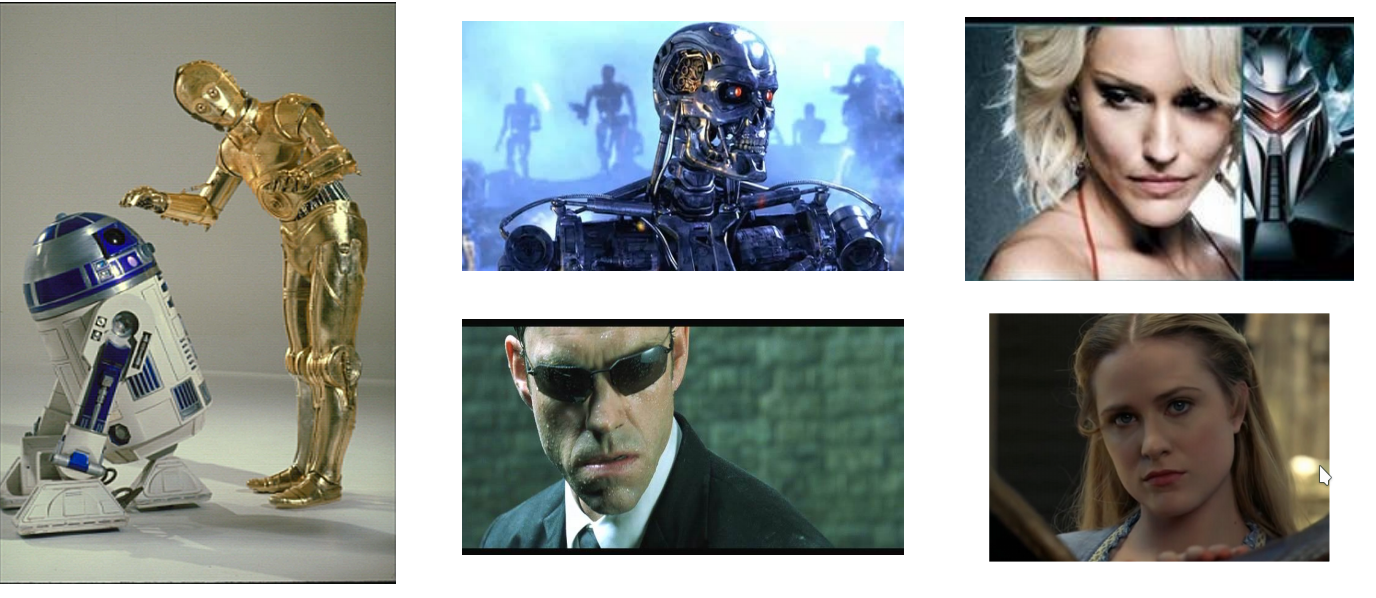
\includegraphics[width=1\textwidth]{img/ia1}
    \end{figure}

\end{frame}

\subsection{Inteligencia Artificial}
\begin{frame}{¿Inteligencia Artificial?}

    \begin{columns}
        \begin{column}{0.32\textwidth}
            \begin{figure}[!h] 
                \centering
                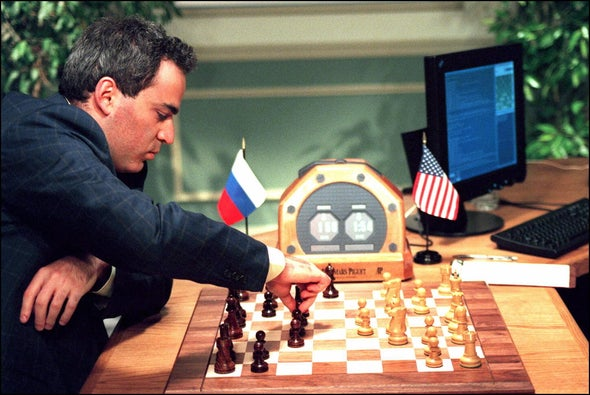
\includegraphics[width=1\textwidth]{img/deepblue}
            \end{figure}                
        \end{column}
        \begin{column}{0.32\textwidth}
            \begin{figure}[!h] 
                \centering
                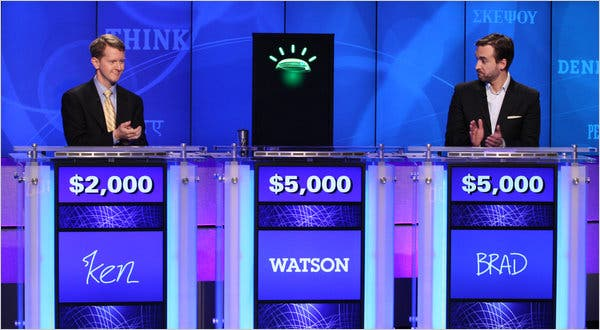
\includegraphics[width=1\textwidth]{img/watson}
            \end{figure}                
        \end{column}
        \begin{column}{0.32\textwidth}
            \begin{figure}[!h] 
                \centering
                
\includegraphics[width=1\textwidth]{img/alphago}
            \end{figure}                
        \end{column}
    \end{columns}
    
\end{frame}

\begin{frame}
    \frametitle{Decisiones Racionales}
    Es un campo de la ciencia que estudia e intenta desarrollar sistemas 
    capaces de tomar decisiones racionales imitando la inteligencia humana (animal).

    El término \alert{racional} se entiende en un contexto técnico como:
    \begin{itemize}
        \item \textbf{Racional} Lograr objetivos predefinidos de manera óptima.
        \item La racionalidad es relativa a las decisiones tomadas (no el proceso detrás).
        \item Los objetivos están expresados en términos de la \alert{utilidad} de lo obtenido.
        \pause
        \item Ser \alert{racional} significa \alert{maximizar la utilidad esperada}.
    \end{itemize}
\end{frame}

\begin{frame}
    \frametitle{En nuestro cerebro}
    \begin{itemize}
        \item Nuestros cerebros son muy buenos tomando decisiones racionales, \alert{pero no perfectos}.
        \item Nuestros cerebros no son modulares (como el software), por tanto son difíciles de analizar.
        \item ``Los cerebros son a la inteligencia lo que las alas son a volar''
        \item Lo que aprendimos de nuestros cerebros: memoria (datos) y simulación (cálculos) son 
        clave para la toma de decisiones.
    \end{itemize}
\end{frame}

\begin{frame}
    \frametitle{En este curso}
    \begin{enumerate}
        \item Inteligencia a partir de cálculos.
            \begin{itemize}
                \item Búsqueda, planificación.
                \item Búsqueda adversaria y bajo incertidumbre.
            \end{itemize}
        \item Inteligencia a partir de datos.
            \begin{itemize}
                \item Algoritmos Genéticos.
                \item Aprendizaje Profundo.
            \end{itemize}
    \end{enumerate}
\end{frame}
\subsection{Historia}
\begin{frame}[allowframebreaks]
    \frametitle{Breve Historia}
    \begin{itemize}
        \item 1940 - 1950:
            \begin{itemize}
                \item Modelo del cerebro con circuito Booleano de McCulluch \& Pitts.
                \item ``Computing Machinery and Intelligence'' de Turing.
            \end{itemize}
        \item 1950 - 1970:
            \begin{itemize}
                \item Programa de Ajedrez de Samuel.
                \item Reunion de Darmouth donde se adopta el término \textit{Inteligencia Artificial}.
                \item Algoritmo completo para razonamiento lógico de Robinson.
            \end{itemize}
        \item 1970 - 1990:
            \begin{itemize}
                \item Sistemas basados en conocimiento.
                \item Sistemas Expertos, ascenso y decadencia. (\textit{Invierno de la IA})
            \end{itemize}
        \item 1990 - 2012:
            \begin{itemize}
                \item Resurgimiento de la probabilidad y foco en incertidumbre.
                \item Sistemas de aprendizaje y agentes \textit{Primavera de la IA}.
            \end{itemize}
        \item 2012 - presente:
            \begin{itemize}
                \item Big data, redes neuronales.
                \item Reunificación de subcampos.
                \item Aprendizaje profundo y el boom de la IA.
            \end{itemize}
    \end{itemize}
\end{frame}
\subsection{Aplicaciones}
\begin{frame}
    \frametitle{Capacidades de la IA - Quiz}
    \begin{itemize}
        \item Jugar una partida decente de tenis de mesa. ( )
        \item Conducir de forma segura por una carretera en una montaña. ( )
        \item Conducir de forma segura por la ciudad. ( )
        \item Comprar una semana de abarrotes en internet. ( )
        \item Comprar una semana de abarrotes en el mercado. ( )
        \item Descubrir un nuevo teorema matemático. ( )
        \item Conversar con una persona de manera exitosa por una hora. ( )
        \item Realizar una operación quirúrgica exitosa. ( )
        \item Traducir Mandarin hablado a inglés hablado en tiempo real. ( )
        \item Doblar la ropa y lavar los platos. ( )
        \item Escribir una historia intencionalmente graciosa. ( )
    \end{itemize}
\end{frame}

\begin{frame}
    \frametitle{Capacidades de la IA}
    \begin{itemize}
        \item Jugar una partida decente de tenis de mesa.   (\checkmark)
        \item Conducir de forma segura por una carretera en una montaña. (\checkmark)
        \item Conducir de forma segura por la ciudad.   (X)
        \item Comprar una semana de abarrotes en internet.(\checkmark)
        \item Comprar una semana de abarrotes en el mercado.X)
        \item Descubrir un nuevo teorema matemático.(X)
        \item Conversar con una persona de manera exitosa por una hora.(X)
        \item Realizar una operación quirúrgica exitosa.(?)
        \item Traducir Mandarin hablado a inglés hablado en tiempo real.(\checkmark)
        \item Doblar la ropa y lavar los platos.(X)
        \item Escribir una historia intencionalmente graciosa.(X)
    \end{itemize}
\end{frame}

\begin{frame}
    \frametitle{Lenguaje Natural}
    Tecnologías del habla:
    \begin{itemize}
        \item Reconocimiento automático de voz (ASR).
        \item Síntesis Texto a Voz (TTS).
        \item Sistemas de diálogo.
    \end{itemize}
    Procesamiento de lenguaje:
    \begin{itemize}
        \item Respuestas naturales.
        \item Traducción.
        \item Búsqueda en la web.
        \item Clasificación de textos.
    \end{itemize}
    
\end{frame}

\begin{frame}
    \frametitle{Visión}
    Pixeles -> Información / Decisión.

    \begin{itemize}
        \item Detección y reconocimiento de objetos.
        \item Segmentación Semántica.
        \item Entendimiento 3D.
    \end{itemize}
\end{frame}

\begin{frame}
    \frametitle{Robótica}
    Mitad Ingeniería mecánica, Mitad IA. El mundo real es mucho mas difícil que las simulaciones.

    \begin{itemize}
        \item Percepción.
        \item Planeamiento y control
        \item Monitoreo e interfaces humano - máquina.
    \end{itemize}
\end{frame}

\begin{frame}
    \frametitle{Juegos}
    \begin{itemize}
        \item 1997: Gary Kasparov cae ante DeepBlue.
        \item 2016: AlphaGo vence a Lee Sedol.
        \item 2019: OpenAI Five vence a un equipo top de Dota 2.
    \end{itemize}
\end{frame}


\begin{frame}
    \frametitle{Presencia de la IA en nuestras vidas}
    La IA aplicada está presente a diario en nuestras vidas en las siguientes aplicaciones:

    \begin{itemize}
        \item Motores de búsqueda.
        \item Planeamiento de rutas.
        \item Logística e inventarios.
        \item Diagnósticos médicos.
        \item Servicios de soporte automatizado.
        \item Detección de Spam y fraude.
        \item Recomendaciones de productos.
        \item Traducción y procesamiento de textos.
        \pause
        \item ... Y mucho más!
    \end{itemize}
\end{frame}


{\setbeamercolor{palette primary}{fg=black, bg=yellow}
\begin{frame}[standout]
  Preguntas?
\end{frame}
}

\appendix

% \begin{frame}[fragile]{Backup slides}
%   Sometimes, it is useful to add slides at the end of your presentation to
%   refer to during audience questions.

%   The best way to do this is to include the \verb|appendixnumberbeamer|
%   package in your preamble and call \verb|\appendix| before your backup slides.

%   \themename will automatically turn off slide numbering and progress bars for
%   slides in the appendix.
% \end{frame}

\begin{frame}[allowframebreaks]{Referencias}
.
\end{frame}

\end{document}
